%%%%%%%%%%%%%%%%%%%%%%%%%%%%%%%%%%%%%%%%%%%%%%
%                                            %
%    Dyussenov Nuraly BSc Thesis Work        %
%                                            %
%%%%%%%%%%%%%%%%%%%%%%%%%%%%%%%%%%%%%%%%%%%%%%

\documentclass[12pt,a4paper,oneside]{book} % twoside,openany

% Packages
\usepackage[T1]{fontenc}
\usepackage[utf8]{inputenc}

\usepackage{amsmath,amssymb,amsthm}
\DeclareMathOperator{\spn}{span}
\usepackage{cancel}
\usepackage{enumerate}
\usepackage{graphicx}
\usepackage{caption,subcaption}
\graphicspath{{./figures/}}

\usepackage{array}
\newcolumntype{L}[1]{>{\raggedright\let\newline\\\arraybackslash\hspace{0pt}}m{#1}}
\newcolumntype{C}[1]{>{\centering\let\newline\\\arraybackslash\hspace{0pt}}m{#1}}
\newcolumntype{R}[1]{>{\raggedleft\let\newline\\\arraybackslash\hspace{0pt}}m{#1}}

\usepackage{url  }
\usepackage{hyperref}
\usepackage{tikz}
\usetikzlibrary{decorations.pathreplacing}
\usepackage{tikz-3dplot}
\usetikzlibrary{calc}

\setlength {\marginparwidth }{2cm}

\usepackage{accents}

\usepackage{todonotes}

\usepackage{setspace}

% code snippets
\usepackage{minted}  
\usepackage{mdframed}


% Theoremlike environment
\newtheorem{theorem}{Theorem}[section]
\newtheorem{proposition}[theorem]{Proposition}
\newtheorem{lemma}[theorem]{Lemma}
\newtheorem{corollary}[theorem]{Corollary}
\newtheorem{remark}[theorem]{Remark}
\newtheorem{definition}[theorem]{Definition}
\newtheorem{example}[theorem]{Example}
\newtheorem{assumption}[theorem]{Assumption}

% Ususal abbreviations
\newcommand{\N}{\mathbb{N}}
\newcommand{\Z}{\mathbb{Z}}
\newcommand{\Q}{\mathbb{Q}}
\newcommand{\R}{\mathbb{R}}

% Probability theory
\newcommand{\A}{\mathcal{A}}
\newcommand{\B}{\mathcal{B}}
\newcommand{\C}{\mathcal{C}}
\newcommand{\F}{\mathcal{F}}
\newcommand{\G}{\mathcal{G}}
\newcommand{\X}{\mathcal{X}}
\newcommand{\Y}{\mathcal{Y}}
\newcommand{\M}{\mathcal{M}}
\renewcommand{\P}{\mathbb{P}}
\newcommand{\E}{\mathbb{E}}
\newcommand{\D}{\mathbb{D}}
\newcommand{\law}[1]{\text{Law}(#1)}

\newcommand{\Var}{\mathrm{Var}}

\newcommand{\Cov}{\mathrm{Cov}}

\newcommand{\Pas}{\text{a.s.}}
\newcommand{\ind}{\mathds{1}}

% Analysis
\newcommand{\eps}{\varepsilon}
\newcommand{\la}{\lambda}
\newcommand{\ga}{\gamma}
\newcommand{\ka}{\kappa}
\newcommand{\dtv}{d_{\text{TV}}}

% Integration
\newcommand{\dint}{\mathrm{d}} 

\newcommand{\lfrf}[1]{\lfloor #1\rfloor}


%%%%%%%%%%%%%%%%%%%%%%%%%%%%%%%%%%%%55% Page layout
\usepackage{indentfirst}
%\usepackage{fullpage}
\usepackage[a4paper]{geometry}
% \geometry{tmargin=3cm,lmargin=3.5cm,rmargin=2cm}
% manual page formatting
%\setlength{\headsep}{25pt}
\hyphenation{}

% headers and footers
\usepackage{fancyhdr}
\usepackage{mathptmx}

\newcommand\HRule{\rule{\textwidth}{1pt}}

\usepackage{varwidth}

%\usepackage{booktabs}
\usepackage{multirow,array}
\usepackage{siunitx}

% Quotations
\usepackage{csquotes}

\makeatletter
\renewcommand{\@chapapp}{}% Not necessary...
\newenvironment{chapquote}[2][2em]
{\setlength{\@tempdima}{#1}%
	\def\chapquote@author{#2}%
	\parshape 1 \@tempdima \dimexpr\textwidth-2\@tempdima\relax%
	\itshape}
{\par\normalfont\hfill--\ \chapquote@author\hspace*{\@tempdima}\par\bigskip}
\makeatother



\newcommand{\code}[1]{\texttt{#1}}


\usepackage{titlesec, blindtext, color}
\definecolor{gray75}{gray}{0.75}
\newcommand{\hsp}{\hspace{20pt}}


\newcommand{\stdwidth}{0.61\linewidth}

% Space above chapter titles
\usepackage{titlesec}

\renewcommand{\baselinestretch}{1.5}



\begin{document}
\onehalfspacing

\begin{titlepage}
	
	%\newcommand{\HRule}{\rule{\linewidth}{0.5mm}} % Defines a new command for the horizontal lines, change thickness here
	
	\center % Center everything on the page
	
	%----------------------------------------------------------------------------------------
	%	HEADING SECTIONS
	%----------------------------------------------------------------------------------------
	
	\textsc{\LARGE Budapesti University of Technology and Economics}\\[1.5cm] % Name of your university/college
	\textsc{\Large Institute of Mathematics}\\[0.5cm] % Major heading such as course name
	\textsc{\large Bachelor Thesis}\\[0.5cm] % Minor heading such as course title
	
	%----------------------------------------------------------------------------------------
	%	TITLE SECTION
	%----------------------------------------------------------------------------------------
	
	\HRule \\[0.4cm]
	{ \Large \bfseries Linear Regression through Origin
		 }\\[0.4cm]
	\HRule \\[1.5cm]
	
	%----------------------------------------------------------------------------------------
	%	AUTHOR SECTION
	%----------------------------------------------------------------------------------------
	
	\begin{tabular}{L{6cm} R{8cm}}
	\emph{Author:}   & \emph{Supervisor:} \\
	Dyussenov Nuraly & Dr. Jozsef Mala   \\
	                 & Associate Professor, BME Fac. of Nat. Sci. 
	\end{tabular}\\[1.3cm]

	
	\vfill
	{\Large Budapest, \today}\\[1.2cm] % Date, change the \today to a set date if you want to be precise
		
	\includegraphics[trim={0cm 0cm 0cm 0cm},clip,width=0.5\linewidth]{bme_logo_nagy.eps}
	 % Include a department/university logo - this will require the graphicx package
	
	%\vfill % Fill the rest of the page with whitespace
	
\end{titlepage}

	%\newpage\null\thispagestyle{empty}\newpage

	\frontmatter
	%\chapter*{\centering Kivonat}
	
	\setcounter{tocdepth}{1}
	\tableofcontents
	\listoftables
	\listoffigures
		
	\mainmatter
	
	\fancypagestyle{plain}{%

		\fancyhf{}
		\fancyhead[L]{\rule[-2ex]{0pt}{2ex}\small \leftmark} 
		\fancyhead[R]{} 
		\fancyfoot[L]{}
		\fancyfoot[C]{-- \thepage\ --}
		\fancyfoot[R]{} 
		\renewcommand{\headrulewidth}{1.5pt}
		\renewcommand{\footrulewidth}{1pt}}
	\pagestyle{plain}
	
	\titleformat{\chapter}[display]{\normalfont\huge\bfseries}{\chaptertitlename\ \thechapter}{20pt}{\Huge}
	\titlespacing*{\chapter}{10pt}{20pt}{40pt}
	 
	\titleformat{\chapter}[hang]{\Huge\bfseries}{\thechapter.\hsp}{0pt}{\Huge\bfseries} 
	  
	\chapter{Introduction}
			
	\section{Background}
	In the world of regression analysis, choosing the right model is a constant challenge, balancing simplicity and accuracy. This thesis focuses on a specific aspect—linear regression through the origin (RTO)—examining its statistical properties when dealing with just one explanatory variable. Our goal is to identify situations where this approach might be more suitable than the commonly used simple linear regression. Through this study, we aim to shed light on the conditions that make regression through the origin a preferable choice, offering insights that bridge mathematical rigor with real-world applicability. Join us on this journey as we navigate the complexities of statistical modeling, striving to understand when and why regression through the origin might outperform its more conventional counterpart.
	
	\section{Literature Review}
	Gerald J. Hahn \cite{hahn1977fitting} published an article on fitting models with no intercept term. In their paper, they focused on the appropriateness of the no-intercept linear regression model in different scenarios. For example, while the physical nature of sample data might advocate for the use of a no-intercept model, it often happens that the true nature of the data is not linear. Extrapolation of the data to the region that falls outside the range of the sample makes it clear that other models should be used. They also provide a procedure for checking the significance of the intercept: one must fit the intercept model and then construct a confidence interval that contains the true intercept, and then check whether 0 is included in the interval. If it is included, then there is no evidence that the intercept model provides a significantly better fit to the data than the no-intercept model. Hahn also raised an issue related to the coefficient of determination that was erroneously computed in popular computing packages of that time.
	
	Gordon \cite{gordon1981errors} has also contributed to the dispute over the computation of $R^2$ and suggested that this parameter has to be computed for both models using the same formula
	
	\begin{equation} \label{eq:coefficient_of_determination}
		R^2 = 1 - \frac{\sum_i \epsilon_i ^2}{\sum_i (y_i-\bar{y})^2}
	\end{equation}
	
	However, as Eisenhauer \cite{eisenhauer2003regression} noted, the equation \ref{eq:coefficient_of_determination} might be inconsistent for the no-intercept model and provide an uninterpretable negative result. So, a different formula for the no-intercept model is commonly used:
	
	\begin{equation}
		R^2 = \frac{\sum \hat{y_i}^2}{\sum y_i^2}
	\end{equation}
	
	This new formula is not consistent with the prior one; thus, $R^2$ calculated for intercept and no-intercept models are incomparable.
	
	\section{Research Question}
	The main goal of this paper is to familiarize the reader with linear regression through the origin, derive properties of its estimators, compare RTO with the full linear regression model with an intercept, and determine when RTO might outperform the full OLS model.
	
	\section{Outline}
	We will start with a recap of some statistical notions that are fundamental to the topic of discussion. Then, we will go through the necessary conditions of OLS regression and connect the notion of least squares with maximum likelihood. After that, we will derive properties of linear regression for both intercept and no-intercept models, and lastly, provide an example of the case when the no-intercept model is better than the full model and try to explain why.
	
	\chapter{Preliminaries}


	\section{Statistics Basics}
	
	In this part we will cover most of the statistics that we are going to need later and also some of the notations that we are going to use.
	
	

\textbf{Definition (Data):} Let $(x_1, \ldots, x_n)$, where $x_i \in S$ for $i = 1, \ldots, n$. The set $S$ is typically $\mathbb{R}$, $\mathbb{R}^d$, or any abstract set. However, for our purposes, $S$ (the sample space) is usually taken as $\mathbb{R}$.

\textbf{Definition (Sample):} In statistics, our data are often represented by a vector $\mathbf{X} = (X_1, X_2, \ldots, X_n)$ of i.i.d. (independent, identically distributed) random variables, denoted as the sample (of size $n$). The random variables $X_i$ take values in $\mathbb{Z}$ or $\mathbb{R}$. The common distribution of the $X_i$ is referred to as the parent distribution, and the sample is said to be drawn from that parent distribution.

\textbf{Definition (Model):} A statistical model is a family $\{P_{\theta} \,|\, \theta \in \Theta\}$ of distributions on the sample space. In the case where $\Theta \subset \mathbb{R}^d$, it is a parametric model, with $\Theta$ being the parameter set (space).

\textbf{Definition (Statistic):} A statistic $T=T(x_1,...,x_n )$ is any function of the sample data, often used to summarize or draw inferences about the underlying population.

\textbf{Definition (Sample mean):} Let $(X_1, \ldots, X_n)$ be a sample. Then, the random variable
\[ \bar{X} = X = \frac{1}{n} \sum_{i=1}^{n} X_i \]
is referred to as the sample mean.

\textbf{Definition (Estimator):} An estimator is a statistic (a function of the sample data) used to estimate an unknown parameter in a statistical model. Denoted as $\hat{\theta}$, an estimator for the parameter $\theta$ is any measurable function of the random variables $X_1, X_2, \ldots, X_n$.

\textbf{Definition (Unbiased Estimator):} If $\hat{\theta}$ is an estimator of $\theta$, we can define the quantity \textit{Bias}($\hat{\theta}$) = $\mathbb{E}_{\theta}[\hat{\theta}] - \theta$. The estimator $\hat{\theta}$ is termed unbiased if its bias is 0.

\textbf{Definition (MSE of an Estimator):} Consider the model $\{P_{\theta} \,|\, \theta \in \Theta\}$ and the sample $(X_1, \ldots, X_n)$ from it. The mean square error (or quadratic risk) of an estimator $\hat{\theta} = \hat{\theta}(X_1, \ldots, X_n)$ for the parameter $\theta$ is defined as
\[ \text{MSE}_{\theta}(\hat{\theta}) = \mathbb{E}_{\theta}((\hat{\theta} - \theta)^2) \]
when $\theta$ is the true parameter.

\textbf{Definition (Likelihood):} We say that $L(\theta)$ is a likelihood of an estimator $\theta$ if $L(\theta)=p(x|\theta)$, where $x$ is a realization $(x_1,...,x_n)$ of a sample $X$. Thus, likelihood can be obtained by taking the product of marginal probability mass functions for fixed $x$, and expressing the result as a function of $\theta$.

\begin{equation} \label{eq:likelihood}
	p(x|\theta) = \Pi^n_{i=1} p(x_i| \theta)
\end{equation}


We will call estimator $\hat{\theta}$ a Maximum Likelihood Estimator of $\theta$ if it maximizes \ref{eq:likelihood}. One common approach to find this estimator is to take partial derivative with respect to $\theta$ of log-likelihood function $l(\theta)=\log L(\theta)$. Since logarithm is a monotonically increasing function, the maximum of $l(\theta)$ will be the same as maximum of $L(\theta)$


\textbf{Remark:} For the sake of convenience, the summation operator and summands will frequently be expressed without an explicit index. The index will only be specified when its omission might cause confusion.

For example:
\[
	\sum (x-\bar{x}) 
\]
Is equivalent to:

\[
	\sum_{i=1} (x_i-\bar{x})
\]



	\chapter{Simple Linear Regression}
	
	
\section{Simple linear regression}

Before we start delving into RTO, it's best to get familiar with a more general case - Simple Linear Regression.

In Simple Linear Regression, we are given a random sample of data points $(x_1,y_1),...,(x_n,y_n)$ from a population, and our goal is to find a linear function that describes the relationship between $x$ (often called, explanatory variable, regressor) and $y$ (often called dependent variable, regressand) as good as possible: 


\begin{equation}\label{eq:lin}
	y_i = \beta_1 x_i + \beta_0 \quad (i= 1,2,...,n)
\end{equation}

or in matrix notation 
\begin{equation*}
	\mathbf{Y} = \mathbf{\beta} \mathbf{X}
\end{equation*}


where  $\mathbf{Y} = 
\begin{bmatrix}
	y_1\\
	y_2 \\
	\vdots \\
	y_n
\end{bmatrix},
\quad
\mathbf{X} = 
\begin{bmatrix}
	1 & x_1 \\
	1 & x_2 \\
	\vdots & \vdots \\
	1 & x_n
\end{bmatrix}, \quad
\mathbf{\beta} =
\begin{bmatrix}
	\beta_0 & \beta_1
\end{bmatrix}
$



Since, sample is random, the equation \eqref{eq:lin} is not true in general, so we take into account error term $\epsilon = (\epsilon_1, \epsilon_2, ... , \epsilon_n)^T$, where $\epsilon_1, \epsilon_2, ... , \epsilon_n$ are i.i.d random variables:

\begin{equation}\label{eq:linear regression} 
	\mathbf{Y} = \mathbf{\beta} \mathbf{X} + \epsilon
\end{equation}


\section{Assumptions}
The objective of simple linear regression is, under some assumption \cite[p.4-12]{hayashi2011econometrics}, to estimate the parameters $\beta_0$ and $\beta_1$, so that they will provide best fit. The assumptions are important since they serve as a foundation for later theory, so it is crucial to know them.

\begin{assumption}[\textbf{linearity}]
	$y_i = \beta_1 x_i+\beta_0 +\epsilon_i$
\end{assumption}

Linearity means that the underlying relationship between regressand and regressor is linear. 

\begin{assumption}[\textbf{strict exogeneity}]
	$\E (\epsilon_i | \mathbf{X})=0 \quad (i=1,2,...,n)$ 
\end{assumption}

From this assumption it follows that:

\begin{equation}
\E (\epsilon_i ) =0 \quad (i=1,2,...,n)
\end{equation}

\begin{proof}
	From law of total expectation it follows that $\E (\epsilon_i ) = \E (\E (\epsilon_i | \mathbf{X}))=0$
\end{proof}

The cross moments are orthogonal to all observations:
\begin{equation}
	\E (x_i \epsilon_j)=0  \quad (i,j = 1, 2, ..., n) 
\end{equation}

\begin{proof}
	\begin{align*}
		\E (x_i \epsilon_j) &= \E (\E(x_i \epsilon_j| x_i))\tag*{(by law of total expectation)} \\
		& =\E (x_i\E( \epsilon_j| x_i)) \tag*{(by linearity of expectation)} \\
		&= \E (x_i 0) 	= 0
	\end{align*}
\end{proof}

Because the mean of error terms is zero, the orthogonality condition, implies that error terms have zero correlation with observations.

\begin{assumption}[\textbf{No collinearity}]
	Vector $(x_1, x_2,...,x_n)$ is not collinear with constant $\mathbf{1}$ vector with probability 1
\end{assumption}

The more general variant of this assumption, in the case when we have classical linear regression with multiple regressors, is no multicollinearity. No multicollinearity would mean that the rank of the $n \times K$ data matrix $\mathbf{X}$ is exactly $K$ with probability 1. In other words, columns of the data matrix have to be linearly independent with probability 1.

\begin{assumption}[\textbf{homoskedasticity}]
	$\E(\epsilon_i^2| \mathbf{X}) = \sigma^2 > 0 \quad (i=1,2,...,n)$
\end{assumption}

\begin{assumption}[no correlation between observatoins]
	\[\E (\epsilon_i \epsilon_j) = 0 \quad (i,j = 1, 2, ..., n; i \neq j) \]
\end{assumption}

This is equivalent to saying that covariance of error terms is zero, since means are zero.

\textbf{Remark:} Although in the assumptions we treat regressors as random, conditioned on their observed values, in reality, $x_1, ..., x_n$ are realizations of random variables, so it is generally accepted to treat them as fixed. Although this might be somewhat misleading, it allows us to shorten the notation, and make it more readable, while still being concise.

For the purposes of this paper, we will also assume that error terms in eq. \ref{eq:linear regression}  are normally distributed with mean 0 and variance $\sigma^2$.

\section{Properties}

To compute likelihood function, we can notice that $y_i$ is a normally distributed random variable with mean $\E [y_i] = \beta_1 x_i + \beta_0$ and variance $\Var \ y = \sigma^2$. Then, likelihood $L$ can be computed as a product of marginal distributions:

\begin{align}
	L(y_1, \ldots, y_n | \beta_0, \beta_1, \sigma) &= \prod \frac{1}{\sqrt{2 \pi \sigma^2}} \exp (-\frac{1}{2\sigma^2}(y_i-(\beta_1 x_i + \beta_0)^2))\\
	&= \left( \frac{1}{2\pi\sigma^2} \right)^{n/2} \exp\left( -\frac{1}{2\sigma^2} \sum_{i=1}^{n} (y_i - (\beta_0 + \beta_1 x_i))^2 \right)
\end{align}


Log-likelihood function
\begin{equation} \label{eq:loglikelihood}
	l(y_1, \ldots, y_n | \beta_0, \beta_1, \sigma) = -\frac{n}{2} \log (2 \pi) - n \log \sigma - \frac{1}{2\sigma^2} \sum_{i=1}^{n} (y_i - (\beta_0 + \beta_1 x_i))^2
\end{equation}

By taking partial derivatives with respect to our parameters, we can find that estimates of $\beta_0, \beta_1$ and $\sigma$ that maximize the likelihood:

% Equations
\begin{align}
	\frac{\partial l}{\partial \beta_0} &= \sum_{i=1}^{n} (y_i - (\beta_0 + \beta_1 x_i)) = 0 \label{eq:est_beta_0} \\
	\frac{\partial l}{\partial \beta_1} &= \sum_{i=1}^{n} (y_i - (\beta_0 + \beta_1 x_i))x_i = 0 \label{eq:est_beta_1} \\
	\frac{\partial l}{\partial \sigma} &= \frac{n}{\sigma} - \frac{1}{\sigma^3} \sum_{i=1}^{n} (y_i - (\beta_0 + \beta_1 x_i))^2 = 0 
\end{align}
	

% Text
Let the solutions of the above equations be denoted as $\hat{\beta}_0$, $\hat{\beta}_1$, $\hat{\sigma}^2$ for $\beta_0$, $\beta_1$, $\sigma^2$. If $\hat{y}_i = \hat{\beta}_0 + \hat{\beta}_1 x_i$ and $S_{xx}= \sum (x-\bar{x})^2, S_{xy}=\sum (x-\bar{x})y$, then...

% Equations
\begin{align}
\hat{\beta}_0  &= \bar{y} - \hat{\beta}_1 \bar{x}; \label{est:intercept} \\
\hat{\beta}_1 &= \frac{S_{xy}}{S_{xx}}; \label{est:slope}\\
\hat{\sigma}^2 &= \frac{1}{n} \sum_{i=1}^{n} (y_i - \hat{y}_i)^2 = \frac{1}{n} SSE.
\end{align}

So $\hat{\beta}_0, \hat{\beta}_1$ are Maximum Likelikelihood Estimators of the model.

\begin{proposition}
	Finding values of $\beta_0, \beta_1 $ that minimize MSE is same as finding MLE of $\beta_0 ,\beta_1 $
\end{proposition}


\begin{proof}
	From equations \ref{eq:est_beta_0} and \ref{eq:est_beta_1} we can see that $y-\hat{y}$ is perpendicular to both $\mathbf{1}$ and $\mathbf{x}$, and we know that $\hat{y}=\hat{\beta_1}x+\hat{\beta_0}$, i.e. $\hat{y}$ lies in $\spn \{ \mathbf{1}, \mathbf{x} \}$.
	Notice that $y-\hat{y}=\epsilon$, so since $\hat{y}$ is perpendicular to $\epsilon$, MLE from \ref{est:intercept} and \ref{est:slope} are indeed MSE estimators too.
\end{proof}


\begin{figure}
	\centering
	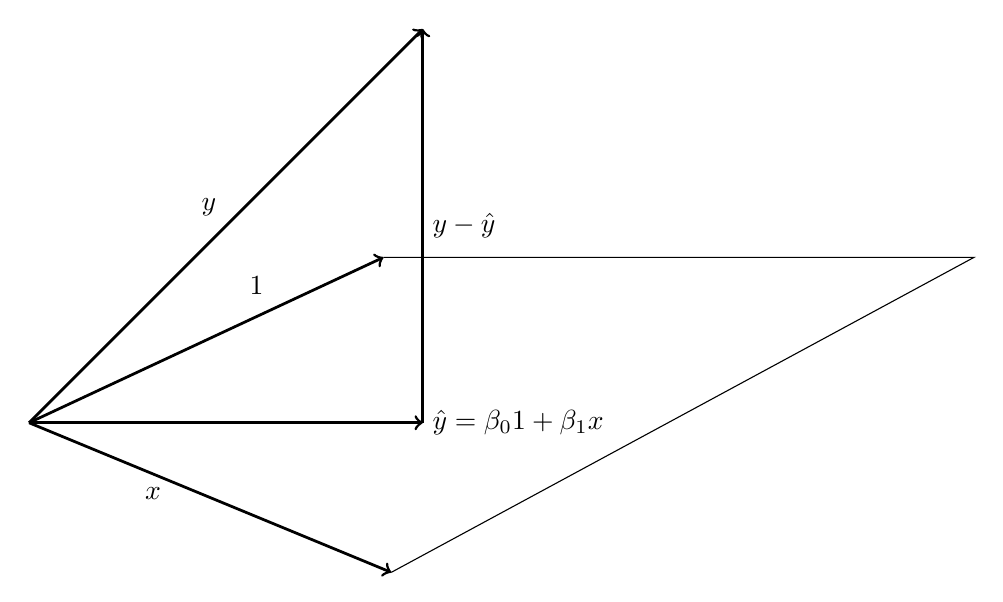
\begin{tikzpicture}
	\draw[->,line width=1] (0,0)--(5,0);
	\draw[->,line width=1] (0,0)--(5,5);
	\draw[->,line width=1] (5,0)--(5,5);
	\draw[->,line width=1] (0,0)--(4.6,-1.9);
	\draw[->,line width=1] (0,0)--(4.5,2.1);
	\draw (4.5,2.1)--(12,2.1)--(4.6,-1.9);
	\node[right] at (5,0) {$\hat{y}=\beta_01+\beta_1x$};
	\node[above left] at (2.5,2.5) {$y$};
	\node[above left] at (3.1,1.5) {$1$};
	\node[below left] at (1.8,-.7) {$x$};
	\node[right] at (5,2.5) {$y-\hat{y}$};
	\end{tikzpicture}
	\caption{Orthogonal projection of $\mathbf{y}$ to $\spn \{ \mathbf{1,x} \}$}
	\label{fig:projection}
\end{figure}%




\textbf{Remark:} Equations \ref{eq:est_beta_0} and \ref{eq:est_beta_1} are called normal equations \cite{neter1983applied} (from the fact that $\mathbf{y-\hat{y}}$ are orthogonal to \textbf{1} and $\mathbf{x}$) and in matrix form it could be written as:

\begin{equation} \label{eq:matrix_form_ols}
	\mathbf{X^TXb = X^TY}
\end{equation}

Where $\mathbf{b}$ is $2 \times 1 $ vector of the regression MLE coefficients $(\hat{\beta_0}, \hat{\beta_1})^T$ 


% Proposition and Proof
\begin{proposition} \label{prop:sst_equation}
	$\underbrace{\sum_{i=1}^{n} (y_i - \bar{y})^2}_{SST} = \underbrace{\sum_{i=1}^{n} (\hat{y}_i - \bar{y})^2}_{SSR} + \underbrace{\sum_{i=1}^{n} (y_i - \hat{y}_i)^2}_{SSE}$
\end{proposition}


% Proof (continued)
\begin{proof}The vector $\textbf{y} - \textbf{$\hat{y}$}$ is perpendicular to $\textbf{$\hat{y}$} - \textbf{1 $\bar{y}$}$, thus the proposition is true by the Pythagorean theorem.

Alternatively, it is enough to show that

\[
	\sum (\hat{y}_i-\bar{y})(y_i-\hat{y}_i) = 0	,
\] since then:

\begin{align*}
	\sum_{i=1}^{n} (y_i - \bar{y})^2 &= (\sum_{i=1}^{n} (\hat{y}_i - \bar{y}) + \sum_{i=1}^{n} (y_i - \hat{y}_i))^2 = \\
	&= \sum_{i=1}^{n} (\hat{y}_i - \bar{y})^2 + 2\sum (\hat{y}_i-\bar{y})(y_i-\hat{y}_i)+ \sum_{i=1}^{n} (y_i - \hat{y}_i)^2 = \\
	&= \sum_{i=1}^{n} (\hat{y}_i - \bar{y})^2 + \sum_{i=1}^{n} (y_i - \hat{y}_i)^2 \\
\end{align*}

From \ref{eq:est_beta_0} we know that $\sum (y_i-\hat{y}_i)=0$.
From \ref{eq:est_beta_1} we know that $\sum (y_i-\hat{y}_i)x_i=0$,
$\hat{y}_i = \beta_0 + \beta_1 x_i \Rightarrow x_i = \frac{1}{\beta_1}(\hat{y}_i-\beta_0) \Rightarrow \sum \hat{y}_i (y_i-\hat{y}_i)=0$

Finally, 

\[
	\sum (\hat{y}_i-\bar{y})(y_i-\hat{y}_i) = \sum \hat{y}_i(y_i-\hat{y}_i)-\bar{y}\sum (y_i-\hat{y}_i)=0	
\]


\end{proof}

Conventionally the terms $\sum_{i=1}^{n} (y_i - \bar{y})^2$, $\sum_{i=1}^{n} (\hat{y_i} - \bar{y})^2$, $\sum_{i=1}^{n} (y_i - \hat{y})^2$ are called Sum of Squares Total (SST),
 Sum of Squares due to Regression (SSR), and Sum of Squares Error (SSE), respectively.


% Proposition
\textbf{Proposition 1.4.} The estimators $\hat{\beta}_0$, $\hat{\beta}_1$, $\frac{SSE}{n-2}$ are unbiased estimators of $\beta_0$, $\beta_1$, $\sigma^2$ respectively.



% Proof that the estimators are unbiased
\textbf{Proof:}

1. \textbf{Unbiasedness of $\hat{\beta}_1$:}


\begin{align*}
	\mathbb{E} [ \hat{\beta _1} ] &= \mathbb{E} [\frac{S_{xy}}{S_{xx}}] = \mathbb{E} [\frac{\Sigma (x_i - \bar{x})(y_i-\bar{y})}{\Sigma (x_i-\bar{x})^2}] \\
		&= \mathbb{E} [\frac{\Sigma (x_i - \bar{x})y_i}{\Sigma (x_i-\bar{x})^2}]=
	\frac{\Sigma (x_i - \bar{x})\mathbb{E} [y_i]}{\Sigma (x_i-\bar{x})^2}\\
		&= \frac{\Sigma (x_i - \bar{x})(\beta_0+\beta_1x_i)}{\Sigma (x_i-\bar{x})^2}=	
	\frac{\Sigma (x_i \beta_0 - \bar{x}\beta_0+\beta_1x_i^2-\beta_1x_i\bar{x})}{\Sigma x_i^2-n\bar{x}^2}\\
		&= \frac{\cancel{n\bar{x}\beta_0}-\cancel{n\bar{x}\beta_0}+\Sigma\beta_1x_i^2-n\beta_1\bar{x}^2}{\Sigma x_i^2-n\bar{x}^2}= \frac{(\Sigma x_i^2-n\bar{x}^2)\beta_1}{\Sigma x_i^2-n\bar{x}^2} = \beta_1 
\end{align*}


2. \textbf{Unbiasedness of $\hat{\beta}_0$:}
\[
\mathbb{E}(\hat{\beta}_0) = \mathbb{E}(\bar{y} - \hat{\beta}_1 \bar{x}) = \bar{y} - \bar{x} \mathbb{E}(\hat{\beta}_1) = \frac{1}{n}\mathbb{E}[\Sigma y_i]-\beta_1 \bar{x} =
\] 

\[
	= \frac{1}{n}\mathbb{E}[\Sigma (\beta_0+\beta_1x_i+\epsilon)]-\beta_1 \bar{x} 
	= \frac{1}{n}n\beta_0+\frac{1}{n}n\beta_1\bar{x}-\bar{x}\beta_1=\beta_0	
\]


3. \textbf{Unbiasedness of $\frac{SSE}{n-2}$ as an estimator of $\sigma^2$:}

Define matrix
\[
U=
\begin{bmatrix}
	\frac{1}{\sqrt{n}} & \dots & \frac{1}{\sqrt{n}} \\
	\frac{(x_1-\bar{x})}{\sqrt{S_{xx}}} & \dots & \frac{(x_n-\bar{x})}{\sqrt{S_{xx}}} \\
	\vdots & \vdots & \vdots \\
	\dots & \dots & \dots
\end{bmatrix}
\]

Where all rows after the second one are deterministic such that U is orthogonal, then $UY=Z$, so that: 

$Z_1 = \sqrt{n}\bar{Y}, \ Z_2 = \frac{S_{xy}}{ \sqrt{S_{xx} }} $, \ and \ $Z_j \sim N(0,\sigma^2) \quad (j=3,...,n)$

Let $\sum_i Z_i^2 = \sum_i Y_i^2$. Notice that we can do this, since choice of U was arbitrary up to the orthogonality of the matrix. Then:

\begin{align*}
	\sum y^2 &= \sum (y-\bar{y})^2 + n \bar{y} \\
	&= \sum (\hat{y}-\bar{y})^2 + \sum (y-\hat{y})^2+ n \bar{y}^2 \\
	&= \sum (\hat{\beta_0}+\beta_1 x-\hat{\beta_0}-\hat{\beta_1}\bar{x})^2 + \sum (y-\hat{y})^2+ n \bar{y}^2 \\
	&= \sum (\hat{\beta_1} x-\hat{\beta_1}\bar{x})^2 + \sum (y-\hat{y})^2+ n \bar{y}^2 \\
	&= \hat{\beta_1}^2 \sum ( x-\bar{x})^2 + \sum (y-\hat{y})^2+ n \bar{y}^2 \\
	&= \frac{S_{xy}^2}{S_{xx}}+n \bar{y}2 + \sum (y-hat{y})^2
\end{align*}

Since $\sum y^2 \sim \sigma^2 \chi (n)$, it follows that $\sum (y-\bar{y})^2 \sim \sigma^2 \chi (n-2) $

Hence, $\E [\frac{SSE}{n-2}]= \frac{\sigma^2 (n-2)}{n-2} = \sigma^2 $

\begin{proposition}
	$\mathbb{V}ar[\hat{\beta}_1] = \frac{\sigma^2}{S_{xx}}$
\end{proposition}

\begin{proof}
	Assume, $Y_i \sim N(0, \sigma^2) $
	\[
		\mathbb{V}ar[\hat{\beta}_1] = \mathbb{V}ar (\frac{1}{S_{xx}}\sum (x_i-\bar{x})Y_i) = \frac{1}{S_{xx}^2}\sum \mathbb{V}ar Y_i = \frac{\sigma^2}{S_{xx}}
	\]
\end{proof}

\begin{proposition}
	$\Var [\hat{\beta_0}]= \frac{\sigma^2 S_{xx}^o}{n S_{xx}} $, where $S_{xx}^o=\sum x^2$
\end{proposition}



\begin{proof}
	\begin{align*}
		\Var [\hat{\beta_0}] &= \Var [\bar{y}- \bar{x}\hat{\beta_1}] = \Var [\bar{y}] + \bar{x}^2 \Var [\hat{\beta_1}]- 2\bar{x} \Cov (\bar{y}, \hat{\beta_1}) = \\ 
		\intertext{($\Cov (\bar{y}, \hat{\beta_1})=0$ see Appendix \ref{appendix:covariance_y_bar_beta_hat})}
		&= \frac{1}{n^2}\Var [\sum y] + \bar{x}^2 \frac{\sigma^2}{(x-\bar{x})^2} \\
		&= \frac{\sigma^2}{n}+\bar{x}^2 \frac{\sigma^2}{(x-\bar{x})^2} \\
		&= \frac{\sigma^2 \sum (x-\bar{x})^2}{n \sum (x-\bar{x})^2}+\frac{n \bar{x}^2 \sigma^2}{n \sum (x- \bar{x})^2} \\
		&= \frac{\sigma^2 }{n \sum (x-\bar{x})^2} (\sum (x-\bar{x})^2+n\bar{x}^2) \\
		&= \frac{\sigma^2 \sum x^2}{n \sum (x-\bar{x})^2}
	\end{align*}
\end{proof}

	\clearpage





\chapter{Linear Regression Regression with no intercept term}

	\section{Simple Linear Regression with no intercept term}

	In certain statistical applications, the conventional assumption of a non-zero intercept term ($\beta_0$) in a simple linear regression model may not align with the nature of the data. For example, in economics the cost of production be assumed to be zero, when there is no production, or in physics, when we are describing the relationship between force and the displacement, forced is assumed to be zero, when there is no displacement. In other words, physical nature of our data often bears information about the nature of the true model. 
	
	
	In linear regression through the origin, regression equation takes the form:
	
	\begin{equation}
		\mathbf{y} = \beta_1^o \mathbf{x} + \mathbf{\epsilon},
	\end{equation}
	where $\mathbf{x}^T=(x_1,x_2,...,x_n)$
	
	
	
	Likelihood function $L$ is:
	\begin{align*}
		L(y_1,...,y_n | \beta_1^o, \sigma) &= \prod \frac{1}{\sqrt{2 \pi \sigma^2}} \exp(-\frac{1}{2\sigma^2 (y_i-\beta_1^o x_i)^2}) \\
		&= \frac{1}{(2\pi \sigma^2)^{n/2}}\exp(-\frac{1}{2\sigma^2} \sum (y_i-\beta_1^o x_i)^2)
	\end{align*}

	Log-likelihood $l$ is:

\[
	l(y_1,...,y_n | \beta_1^o, \sigma)=-\frac{n}{2}\log(2\pi \sigma^2)-\frac{1}{2 \sigma^2} \sum (y_i - \beta_1^o x_i)^2
\]

Thus we can compute the maximum likelihood estimator of $\beta_1^o$ by taking partial derivative of log-likelihood with respect to $\beta_1^o$:

\begin{align*}
	\frac{\partial l}{\partial \hat{\beta_1^o}} = - \frac{1}{2 \sigma^2} & \sum 2(y_i-\hat{\beta_1^o} x_i)(-x_i)=0 \\
	\frac{1}{\sigma^2}& \sum (y_i x_i - \hat{\beta_1^o} x_i ^2) = 0 \\
	& \sum x_i y_i =  \sum  x_i^2 \hat{\beta_1^o} \\
	& \hat{\beta_1^o} = \frac{\sum x_i y_i}{\sum x_i^2}
\end{align*}





	\begin{proposition}
		$\hat{\beta}_1^o$ is unbiased
	\end{proposition}
	\begin{proof}
		\begin{align*}
			\mathbb{E} [\hat{\beta_1^o}] &= \mathbb{E} [\frac{\sum x_i y_i}{\sum x_i^2}] = \sum \frac{1}{x_i^2} \mathbb{E}[\sum x_i y_i] = \\
			&= \frac{\sum x_i\mathbb{E}[y_i]}{\sum x_i^2} = \frac{\sum x_i^2 \beta_1^o}{\sum x_i^2} = \beta_1^o 
		\end{align*}
	\end{proof}
	\begin{proposition} \label{prop:variance_slop_no_intercept}	$\mathbb{V}ar[\hat{\beta}_1^0] = \frac{\sigma^2}{\sum x_i^2}$
	\end{proposition}
	\begin{proof}	$
		\mathbb{V}ar[\hat{\beta}_1^0] =  \mathbb{V}ar[\frac{\sum x_i y_i}{\sum x_i^2}] = \frac{1}{(\sum x_i^2)^2} \sum x_i^2 \mathbb{V}ar[Y_i] = \frac{\sigma^2}{\sum x_i^2}
		$
	\end{proof}


	\begin{proposition} \label{prop:variance_no_intercept_is_lower}
		\[
			\mathbb{V}ar[\hat{\beta}_1^0] < \mathbb{V}ar[\hat{\beta}_1]
		\]
	\end{proposition}

	\begin{proof}
		\begin{align*}
			\sum x_i^2 &> \sum (x_i - \bar{x})^2  \\
			\frac{1}{\sum x_i^2}  &< \frac{1}{\sum (x_i - \bar{x})^2}  \\
			\frac{\sigma^2}{\sum x_i^2}  &< \frac{\sigma^2}{\sum (x_i - \bar{x})^2}  \\
			\mathbb{V}ar[\hat{\beta}_1^0] &< \mathbb{V}ar[\hat{\beta}_1] 
		\end{align*}
	\end{proof}

This tells us that when the true intercept is zero, no-intercept model provides better fit, as the two estimators ($\hat{\beta_1}, \hat{\beta_1^o}$) are unbiased, but the latter has smaller variance. 
This might suggest that $\hat{\beta}_1^0$ might be more accurate estimator than $\hat{\beta}_1$ for the slope term. This gives us some motivation to compare the two estimators more closely.

It would be convenient for us to find confidence interval for $\beta_1^0 - \beta_1$, since if 0 lies in the CI, then we can statistically infer that two estimators are very close.

\begin{proposition} \label{prop:normally}
	The difference of the two estimators is normally distributed as follows: 
	\[
		\hat{\beta_1^0}-\hat{\beta_1} \sim N(\beta_1^0-\beta_1, \sigma^2(\frac{1}{S_{xx}}-\frac{1}{S_{xx}^0}))
	\]
\end{proposition}

	Before proving proposition \ref{prop:normally}, let's first understand some properties of $\hat{\beta_1^0}-\hat{\beta_1}$:

\begin{proposition}
	$\Cov (\hat{\beta_1^0},\hat{\beta_1^0}-\hat{\beta_1})=0$
\end{proposition}

\begin{proof}
	\begin{align*}
		\Cov (\hat{\beta_1^0},\hat{\beta_1^0}-\hat{\beta_1}) &=
		\Cov (\frac{\sum xy}{\sum x^2},\frac{\sum xy}{\sum x^2}-\frac{\sum (x-\bar{x})y}{\sum (x-\bar{x})^2})  \\
		&= \frac{\sum x^2}{(\sum x^2)^2} \Var\  y - \frac{\sum x(x-\bar{x})}{\sum x^2 \sum (x-\bar{x})^2} \Var \ y \\
		&=\sigma^2(\frac{1}{\sum x^2} - \frac{\sum x^2 - \bar{x}\sum x}{\sum x^2 \sum(x^2-2x\bar{x}+\bar{x}^2)}) \\
		&= \sigma^2 (\frac{1}{\sum x^2}-\frac{\sum x^2 - n \bar{x}^2}{\sum x^2(\sum x^2 - 2n\bar{x}^2+n\bar{x}^2)}) \\
		&=\sigma^2 (\frac{1}{\sum x^2}-\frac{\sum x^2 - n \bar{x}^2}{\sum x^2(\sum x^2 -n\bar{x}^2)}) \\
		&= \sigma^2(\frac{1}{\sum x^2}-\frac{1}{\sum x^2})=0
	\end{align*}
\end{proof}

\begin{proposition}
	$\E [\hat{\beta_1^0}-\hat{\beta_1}]=\beta_1^0-\beta_1$ 
\end{proposition}

\begin{proof}
	By linearity of expected value, $\E [\hat{\beta_1^0}-\hat{\beta_1}]= \E[\hat{\beta_1^0}] - \E[\hat{\beta_1}]= \beta_1^0-\beta_1 $
\end{proof}

\textbf{Remark:} This is only true when true intercept is equal to zero, since both of the estimators are MLE in this case.
	
	Now we are ready to prove proposition \ref{prop:normally}
\begin{proof}[Proof of prop. \ref{prop:normally}]
	$\hat{\beta_1^0}-\hat{\beta_1}$ is a linear combination of mutually independent normally distributed r.v.-s $\Rightarrow$ it is normally distributed.
	
	
	\begin{align*}
		\Var (\hat{\beta_1^0}-\hat{\beta_1})&=\Var(\hat{\beta_1^0}) + \Var(\hat{\beta_1}) - 2 \Cov (\hat{\beta_1^0},\hat{\beta_1}) =\frac{\sigma^2}{S_{xx}^0}+\frac{\sigma^2}{S_{xx}}-2 \Cov (\hat{\beta_1^0},\hat{\beta_1^0}-\hat{\beta_1})-2 \Cov (\hat{\beta_1^0},\hat{\beta_1^0}) \\
		&= \frac{\sigma^2}{S_{xx}^0}+\frac{\sigma^2}{S_{xx}} - 0 -2 \Var \ \hat{\beta_1^0}=\frac{\sigma^2}{S_{xx}}-\frac{\sigma^2}{S_{xx}^0}
	\end{align*}
\end{proof}
	
Using proposition \ref{prop:normally}, we can now construct confidence interval for $\beta_1^0-\beta_1$:

\[
			\hat{\beta_1^0}-\hat{\beta_1} \sim N(\beta_1^0-\beta_1, \sigma^2(\frac{1}{S_{xx}}-\frac{1}{S_{xx}^0}))
\]

\[
	Z := \frac{\hat{\beta_1^0}-\hat{\beta_1}-\E [\hat{\beta_1^0}-\hat{\beta_1}]}{\Var (\hat{\beta_1^0}-\hat{\beta_1})}= \frac{\hat{\beta_1^0}-\hat{\beta_1}-(\beta_1^0-\beta_1)}{\sigma^2(\frac{1}{S_{xx}}-\frac{1}{S_{xx}^0})})
\]

\[
	\beta_1^0-\beta_1= \hat{\beta_1^0}-\hat{\beta_1} - \sigma^2 Z(\frac{1}{S_{xx}}-\frac{1}{S_{xx}^0})
\]

CI is:

\begin{equation}
\hat{\beta_1^0}-\hat{\beta_1} - \sigma^2 Z_{\alpha}(\frac{1}{S_{xx}}-\frac{1}{S_{xx}^0}) \leq \beta_1^0-\beta_1 \leq \hat{\beta_1^0}-\hat{\beta_1} + \sigma^2 Z_{\alpha}(\frac{1}{S_{xx}}-\frac{1}{S_{xx}^0})
\end{equation}




\section{Model Comparison}

The goal of this section is to compare two models given that the observed data is generated from the function $y_i = \beta_1 x + \beta_0 + \epsilon_i$ with our standard assumptions. 

\subsubsection{Coefficient of Determination}

	$R^2$ or a coefficient of determination is defined as $$R^2= 1 - \frac{SSE}{SST}$$
	Is is often used to measure how well a model predicts an outcome. It is a proportion of variation in the dependent variable that is explained by independent variables.
	
	However, notion of SST and SSR for no-intercept model is different from the full model as defined in prop. \ref{prop:sst_equation}, since $\sum (\hat{y}_i-\bar{y})(y_i-\hat{y}_i)$ will generally take a non-zero value, so the proof of prop. \ref{prop:sst_equation} fails. It is often argued \cite{eisenhauer2003regression} that defining SST as the sum of squared deviations from the mean is inappropriate when the regression line passes through the origin, but does not necessarily pass through $(\bar{x}, \bar{y})$,  therefore equation in prop. \ref{prop:sst_equation} is replaced by:
	
	$$\underbrace{\sum_{i=1}^{n} y_i^2}_{SST} = \underbrace{\sum_{i=1}^{n} \hat{y}_i^2}_{SSR} + \underbrace{\sum_{i=1}^{n} (y_i - \hat{y}_i)^2}_{SSE}$$
	
	Considering the new definition of $SST$ for RTO, it now does not make much sense to use $R^2$ values of RTO and ordinary OLS linear regressions for model comparison. However it still important to mention this, because this measure is widely used and will result in erroneous inferences if one does not realize this subtle difference.

\subsubsection{Akaike Information Criterion}

Akaike Information Criterion is a statistical tool that was introduced by Akaike in 1974 \cite{akaike1974new} and defined as:

\begin{equation*}
	AIC = (-2) \log (\text{maximum likelihood}) + 2 k
\end{equation*}

Where $k$ is the number of independently adjusted parameters within the model.

AIC in a sense estimates the prediction error for a given set of data, and effectively takes into account the number of assumed parameters, thus punishing overfitting, which often occurs due to increasing number of parameters in the model also increases likelihood, even if the model may give a poorer fit.

AIC has its relation to another important notion in statistics, Kullback-Leibler divergence, which is defined as follows:

Given that $x_1, x_2, ..., x_n$ are obtained results after $n$ independent observations of random variable with probability function $g(x)$, and a parametric family of density function is given by $f(x| \theta )$ then the average log-likelihood tends to this integral (assuming that integral exists) with probability 1
\begin{equation}
	S(g; f(.| \theta)) = \int g(x) \log f(x| \theta)dx
\end{equation}
The idea behind using the log function here is that it is the most sensitive to small deviations of $f(x| \theta)$ from $g(x)$. 
Then the difference 
\begin{equation*}
	I(g; f(.|\theta)) = S(g;g) - S(g; f(.|\theta))
\end{equation*}
is called Kullback-Leibner mean information, and also can be interpreted as "distance" between two distributions $f$ and $g$, since $S(g;g) - S(g; f(.|\theta))$ is also 
\[
	\E_{g} [\log g(x)] - \E_{g} [\log f(x|\theta)]
\]

with respect to the density function $g(x)$. Hence, low values of KL divergence indicate that the two probability density functions are relatively close to each other.

Akaike found that maximized log-likelihood is a biased estimate of 
$\E [\log f(x|\hat{\theta)}$,
 where $\hat{\theta}$ is a biased estimate of $\theta$, where bias approximately equals $k$, the overall number of independent parameters of a given model. Since, $\E [\log g(x)]$ is a constant, minimizing AIC means minimizing the estimate of KL divergence. 



\subsubsection{Bayesian Information Criterion}

Bayesian Information Criterion, Schwartz (1978) \cite{schwarz1978estimating},  is alternative estimate of goodness of fit of the model that penalizes the number of independent parameters and defined as:

\begin{equation}
	BIC = -2 \log(\text{maximized likelihood})+ k \log n
\end{equation}

The way how AIC and BIC penalize increasing number of parameters is different, and ultimately the choice between two criterions should depend on assumptions about reality and the intent of the model-based inference \cite{burnham2004multimodel}. However, for the sake of practice, we shall use both AIC and BIC in our model comparison.



\subsection{$\beta_0 = 0:$}

When the true intercept term is equal to zero, for both models we have that their parameters are MLE of true parameters. However, from prop. \ref{prop:variance_no_intercept_is_lower} we know that the slope estimator of the no-intercept model is more accurate, hence no-intercept model is preferred.


\subsection{$\beta_0 \neq 0:$}

It is intuitive to presume that in general, when true intercept term is not equal to zero, intercept model should perform better, as it is unbiased, however the following example might suggest that the no-intercept model is better for small values of $\beta_0$ if we look at the sum of squared deviations of fitted points from the points on the true relationship line:

\[
	\sum (\dot{y}-\hat{y})^2
\]
Where $\dot{y}=\beta_1 x + \beta_0$ and $\beta_0, \beta_1$ are true intercept and slope values, respectively.

	\subsubsection{Motivational example}

Even though RTO might be worse than performing full linear regression model in terms of SSE (since full model always gives unbiased estimators, they are also MLE estimators, so SSE is minimized), there are other statistical parameters that are better in RTO when intercept term is small enough.

Given that the true model is known, $\dot{y_i} = \beta_1 x_i + \beta_0$, one might simulate the data points by adding normally-distributed error terms:

\[
	y_i =  \beta_1 x_i + \beta_0 + \epsilon_i
\]

One might be interested now in comparing sum of squared deviations (SSD) of fitted points $\sum (\dot{y_i}-\hat{y_i})^2 $.

Let's start by generating a sample of 100 points, and assume that parameters are known as $\beta = 1, \alpha = 0.005, \sigma=1$ (see fig. \ref{fig:simulation}):



\begin{figure}
	\begin{subfigure}{0.5\textwidth}
		\centering
		\includegraphics[width=\linewidth]{simulation.png}
		\caption{Plot of simulated points}
		\label{fig:simulation}
	\end{subfigure}%
	\begin{subfigure}{0.5\textwidth}
		\centering
		\includegraphics[width=\linewidth]{threemodels.png}
		\caption{Plot of three models}
		\label{fig:threemodels}
	\end{subfigure}
	\caption{Linear Regression model on simultated datapoints}
\end{figure}


Now, let's fit two models: no-intercept model, and full model. For that purposes we will use LinearRegression function from \code{sklearn.linear\_model} package. On fig. \ref{fig:threemodels} you can see the two models as well as the true model plotted up close (The code for plotting all of the plots can be found in appendix).

\begin{table}
	\centering
	\begin{tabular}{lccc} 
		& AIC & BIC & SSD \\
		Intercept Model & 1102.35 & 1110.16 & 0.46305 \\
		No Intercept Model & 1100.24 & 1105.45 & 0.45767 \\
	\end{tabular}
	\caption{AIC, BIC, and SSD for Intercept and No Intercept Models.}
	\label{tab:model_comparison}
\end{table}

Now let's compare three statistics for these two models: BIC, AIC and SSD. The results can be seen in the Table \ref{tab:model_comparison}. It is clearly seen that no-intercept model provides slightly better fit in terms of these parameters.

Moreover, when we perform 1000 Monte Carlo simulations for 1000 different intercept values $\beta_0$, ranging from 0 to 0.2, and $\beta_1=1, \sigma^2=1$, and we plot the graph of $\Delta SSD := SSD_{no}-SSD$ to $\beta_0$, we can see that $\Delta SSD$ takes negative values in the region that is bellow blue dashed line in fig. \ref{fig:ssd_to_intercept}. This might suggest that no-intercept model is better in terms of SSD compared to the full model. However let's give this assumption a mathematical justification.

\begin{figure}
	\centering
	\includegraphics[width=\linewidth]{delta_ssd_to_intercept.png}
	\caption{Plot of the difference of SSD to the values of intercept}
	\label{fig:ssd_to_intercept}
\end{figure}%

\subsection{Expected value of $SSD$ and $SSD_{no}$}

We will denote with $SSD$ and $SSD_{no}$ the sum of squared deviations of the fitted values from values on the true relationship line for full and no-intercept models, respectively. 

Our goal here is to calculate $\E [SSD]$ and $\E [SSD_{no}]$ to justify the region below zero in fig. \ref{fig:ssd_to_intercept}. In this section we are going to prove the following two propositions:

\begin{proposition} \label{prop:ssd_no_intercept}
	$\E[SSD_{no}] = n \beta_0^2-\beta_0^2n^2 \frac{\bar{x}^2}{\sum x^2}+ \sigma^2$ 
\end{proposition}

\begin{proposition} \label{prop:ssd_full_model}
	$\E [SSD]= \frac{2\sigma^2}{S_{xx}}(S_{xx}^o-n\bar{x}^2)$
\end{proposition}

Assuming $\beta_0 >0$. In order to prove proposition \ref{prop:ssd_no_intercept}, we have to take into account that $\beta_0 \neq 0$, so the estimator $\beta_1^o$ is now biased.

\begin{proposition} \label{prop:expect_slope_term_biased}
	$	\E [\hat{\beta}_1^o]= \frac{\sum \beta_0 x }{\sum x^2} + \beta_1$ 
\end{proposition}

\begin{proof}

\begin{align*}
	\E [\hat{\beta}_1^o] &=\frac{\E \sum xy}{\sum x^2}
	= \frac{\sum x \E[y]}{\sum x^2} 
	=  \frac{\sum x (\beta_1 x + \beta_0) }{\sum x^2} \\
	&= \frac{\sum \beta_0 x + \sum \beta_1 x^2}{\sum x^2} 
= \frac{\sum \beta_0 x }{\sum x^2} + \beta_1
\end{align*}  

\end{proof}


\begin{proposition} \label{prop:expect_slope_term_biased_squared}
	$\E [\hat{\beta_1^o} ^2] = \frac{\sigma^2}{\sum x^2} + (\frac{\sum \beta_0 x}{\sum x^2}+ \beta_1)^2$ 
\end{proposition}

\begin{proof}
	Comes from the fact that $\E [\hat{\beta_1^o} ^2] = \Var [\hat{\beta_1^o}] + \E [\hat{\beta_1^o}]^2 $ and then one can apply prop. \ref{prop:expect_slope_term_biased} and prop. \ref{prop:variance_slop_no_intercept}
\end{proof}


\begin{proof}[Proof of proposition \ref{prop:ssd_no_intercept}]
Here, we assume that $\hat{y}$ are values fitted by no-intercept model:
\begin{align*}
	\E[SSD_{no}] &= \sum (\dot{y} - \hat{y})^2   && \text{\small{(df $SSD_{no}$)}}\\
	&=  \sum \dot{y}^2 - \sum 2 \dot{y} \E [\hat{y}] + \sum \E [\hat{y}^2] && \text{\small{(linearity)}} \\
	& = \sum \dot{y}^2 - \sum 2 \dot{y} x(\frac{\sum \beta_0 x }{\sum x^2} + \beta_1) + \sum x^2 ( \frac{\sigma^2}{\sum x^2}+(\frac{\sum \beta_0 x }{\sum x^2})^2 + \frac{2 \beta_0 \beta_1 \sum x}{\sum x^2} + \beta_1^2) && \text{\small{(pp \ref{prop:expect_slope_term_biased} \& \ref{prop:expect_slope_term_biased_squared})}}\\
	&= \sum (\beta_0^2 + 2 \beta_0 \beta_1 x + x^2 \beta_1^2) - 2x(\beta_0+\beta_1x)(\frac{\sum \beta_0 x }{\sum x^2} + \beta_1)+ \\
	& \quad \sigma^2+\beta_0^2\frac{n^2\bar{x}^2}{S_{xx}^o}+2n\beta_0\beta_1\bar{x}+\beta_1^2S_{xx}^0 \\
	&= n \beta_0^2 + \cancel{2n\beta_0\beta_1\bar{x}}+\cancel{\beta_1^2S_{xx}^o}-2\beta_0^2n^2\frac{\bar{x}^2}{S_{xx}^o}-\cancel{4n\beta_0\beta_1\bar{x}}-\cancel{2\beta_1^2S_{xx}^o}+ \\
	& \quad \sigma^2+\beta^2_0 \frac{n^2 \bar{x}^2}{S_{xx}^o}+\cancel{2n\beta_0\beta_1\bar{x}}+\cancel{\beta_1^2S_{xx}^o} \\
	&= n\beta_0^2-\beta_0^2 n^2 \frac{\bar{x}^2}{S_{xx}^o}+ \sigma^2
\end{align*}

\end{proof}
	
	
Before we begin the proof of proposition \ref{prop:ssd_full_model} let us change our assumptions again, and now let $\hat{y}$ define fitted values by full model.

\begin{proposition} \label{prop:covariance_slope_intercept}
	$\Cov (\hat{\beta_0},\hat{\beta_1})= \frac{-\bar{x} \sigma^2}{\sum (x-\bar{x})^2}$
\end{proposition}
	
\begin{proof}
	Let us adopt matrix notation from equation \ref{eq:linear regression}.
	$Var(\hat{\beta})$ will give us a matrix that has variances of estimators $\hat{\beta_0}, \hat{\beta_1}$ in diagonal elements and their covariances in off-diagonal elements. Define $2 \times 1$ vector $\hat{\beta}$ as $\mathbf{b}$:
	
	\begin{align*}
		\Var [\mathbf{b}] &= \E [\mathbf{b}^2] - \E [\mathbf{b}] \E[\mathbf{b}^T] \\
		&= \E [\mathbf{((X^TX)^{-1}X^TY})^2] - \beta^2 \\
		\intertext{Replace $\mathbf{Y}$ by eq. \ref{eq:linear regression}}
		&= \E [\mathbf{((X^TX)^{-1}X^T(X
			\beta+\epsilon)})^2] - \beta^2 \\
		&= \E [\mathbf{((X^TX)^{-1}X^TX
			\beta+(X^TX)^{-1}X^T\epsilon)})^2] - \beta^2 \\
	\intertext{The term $\mathbf{(X^TX)^{-1}X^TX
	}$ is equal to identity matrix $\mathbf{I_2}$ }
		&=  \E [\mathbf{(\beta+(X^TX)^{-1}X^T\epsilon)})^2] - \beta^2 \\
		&=  \beta^2 + \mathbf{\E [((X^TX)^{-1}X^T\epsilon)^2]} - \beta^2 \\
		\intertext{The cross term becomes zero since $\E [\epsilon]=0$}
		&= \mathbf{((X^TX)^{-1}X^T)^2\E [\epsilon^2]} \\
		&= \mathbf{(X^TX)^{-1}X^TX(X^TX)^T \ ^{-1} \sigma^2} \\
		\intertext{($\mathbf{(X^TX)^T \ ^{-1}= (X^TX)^{-1}}$ comes from the fact that $X^TX$ is a symmetric matrix)}
		&= \sigma^2 (\mathbf{X^TX})^{-1}
	\end{align*}
	
	Now the off-diagonal term then can be computed easily as $\frac{-\bar{x}\sigma^2}{\sum (x-\bar{x})^2}$
	
\end{proof}


\begin{proof}[Proof of proposition \ref{prop:ssd_full_model}]
	\begin{align*}
		\E[SSD] &= \E[\sum (\dot{y}-\hat{y})^2] = \E [\sum (\dot{y}^2 - 2 \dot{y}\hat{y}+\hat{y}^2)]= \\
		&= n \beta_0^2 + 2 \beta_0 \beta_1 \sum x + \beta_1^2 \sum x^2 - \sum 2 \dot{y} \E [\hat{y}] + \sum \E [\hat{y}^2] = (\ast)\\
		\intertext{($\E [\hat{y}] = \E [\hat{\beta_1}]x + \E [\hat{\beta_0}] = \beta_1 x + \beta_0=\dot{y}$)}
		\intertext{$\E[\dot{y}^2]=\Var[\hat{\beta_0}]+\E[\hat{\beta_0}]+x^2(\Var [\hat{\beta_1}+\E [\hat{\beta_1}]^2])+2x\E[\hat{\beta_0}\hat{\beta_1}]$}
		\intertext{and $\E[\hat{\beta_0}\hat{\beta_1}]= \Cov (\hat{\beta_0},\hat{\beta_1})+\E[\hat{\beta_0}]\E[\hat{\beta_0}]$, so substituting prop \ref{prop:covariance_slope_intercept} we get}
		(\ast) &= n \beta_0^2+2\beta_0 \beta_1 n \bar{x} + \beta_1^2 S_{xx}^o - \sum 2(\beta_1x+\beta_0)^2+\frac{\sigma^2 S_{xx}^o}{S_{xx}}+n\beta_0^2+ \frac{\sigma^2 S_{xx}^o}{S_{xx}} + \\
		& \quad +\beta_1^2 S_{xx}^o-\frac{2n\bar{x}^2\sigma^2}{S_{xx}}+2\beta_0\beta_1x \\
		&= n \beta_0^2+2\beta_0 \beta_1 n \bar{x} + \beta_1^2 S_{xx}^o -2\beta_1^2 S_{xx}^o-4\beta_0\beta_1n\bar{x} -2n\beta_0^2+\frac{\sigma^2 S_{xx}^o}{S_{xx}}+n\beta_0^2+ \frac{\sigma^2 S_{xx}^o}{S_{xx}} + \\
		& \quad +\beta_1^2 S_{xx}^o-\frac{2n\bar{x}^2\sigma^2}{S_{xx}}+2\beta_0\beta_1x \\
		&= \frac{2\sigma^2}{S_{xx}}(S_{xx}^o-n\bar{x}^2)
	\end{align*}
\end{proof}

Looking at the expected value of SSD for both models we see that expected SSD for full model is only explained by variance of the error terms, whereas no-intercept model's SSD also depends on the value of true intercept. Therefore for small values of intercept no-intercept model is expected to perform better in terms of sum of squared deviations of fitted values from true values.


\clearpage



		
	\chapter{Summary and closing words}
	
	\section{Conclusion}
	
In this thesis, we have conducted a comparative analysis of several properties between RTO and OLS models. We explored the variances of estimators of the slope, created a confidence interval for the difference of two slope estimators, and determined the average values of the sum of squared deviations of fitted values from true values. Our findings indicate that, on average, for small intercept values, linear regression through the origin provides a better fit.

When we augment the normal OLS assumptions with the additional assumption that the true intercept term is zero, we can confidently assert that RTO is a valid choice between the two models. This is because RTO is unbiased and provides a smaller variance.

Fitting RTO to a dataset generated from a linear function that includes an intercept term revealed that, although RTO produced biased estimators, the bias for very small intercept values can be mitigated by its simplicity. The full model includes an estimate for the intercept term, increasing the overall variability of the model. On the other hand, the no-intercept model lacks this estimate, resulting in a more precise model, even though it is generally less accurate.
	
	
	
	
	
	



	% All in all 26-30 pages
	

	\bibliography{nuraly}
	\bibliographystyle{plain}
	
	\appendix
	
	\chapter{Appendix}
	
	\section{Miscellaneous calculations}
	
	\begin{proposition}  $\Cov (\bar{y}, \hat{\beta_1})=0$ \label{appendix:covariance_y_bar_beta_hat}
	\end{proposition}
	
	\begin{proof}
		\begin{align*}
			\Cov (\bar{y}, \hat{\beta_1}) &= \Cov (\frac{1}{n}\sum_i y_i, \frac{\sum_j (x_j - \bar{x})y_j}{\sum (x - \bar{x})^2})\\
			&= \frac{1}{n} \sum_i \sum_j \frac{x_j-\bar{x}}{\sum_i(x_i - \bar{x})^2} \Cov (y_j , y_i) \\
			&= \frac{1}{n} \sum_i \frac{(x_i - \bar{x})}{\sum_i (x_i-\bar{x})^2}\sigma^2 \\
			&= 0
			\intertext{since $\sum(x_i - \bar{x})=0$}
		\end{align*}
	\end{proof}
	
	\section{linear\_regression.py module}
	
	
\begin{mdframed}[linecolor=black, topline=true, bottomline=true,
	leftline=false, rightline=false, backgroundcolor=yellow!20!white]
	\begin{minted}[mathescape, linenos, fontsize=\small]{python}
	
import numpy as np
import matplotlib.pyplot as plt
from sklearn.linear_model import LinearRegression

def linear_regression(x, y, intercept=True):
"""
facade function that implements LinearRegression from sklearn.linear_model
"""
model = LinearRegression(fit_intercept=intercept)
x = x.reshape(-1,1)
y = y.reshape(-1,1)
model.fit(x,y)
return model.predict(x)

def bayesian_information_criterion(y, y_fit, n , sigma, k):
"""
BIC calculation for OLS
"""
max_log_likelihood = (
-n/2 * np.log(2 * np.pi * sigma**2)-np.sum((y-y_fit)**2)/(2*sigma**2)
)
BIC = k*np.log(n)-2*max_log_likelihood
return BIC

def akaike_information_criterion(y, y_fit, n , sigma, k):
"""
AIC calculation for OLS
"""
max_log_likelihood = (
-n/2 * np.log(2 * np.pi * sigma**2)-np.sum((y-y_fit)**2)/(2*sigma**2)
)
AIC = -2*max_log_likelihood+2*k
return AIC

def SSD(y, y_fit):
"""
function calculates sum of squared deviations of fitted
values and true values
"""
return np.sum((y-y_fit)**2)
	
	\end{minted}
\end{mdframed}
	
	\section{Script 1}
	
The following script plots generates data from given true linear function by adding normally distributed error terms. The result is plotted 
	
\begin{mdframed}[linecolor=black, topline=true, bottomline=true,
	leftline=false, rightline=false, backgroundcolor=yellow!20!white]
\begin{minted}[mathescape, linenos, fontsize=\small]{python}
import numpy as np
import matplotlib.pyplot as plt

np.random.seed(42)

num_samples = 100  # number of sample points

#X = np.linspace(0, 1, num_samples) * 2 - 1
X = np.random.rand(num_samples) * 2 - 1

sigma = 0.5
beta =  1 # true slope
beta_0 = 0.0005
noise = np.random.normal(0, sigma, num_samples)  # standard normal noise term

y = beta * X + noise + beta_0

plt.plot(
X, beta * X, color='red', 
linewidth=1, label='True Linear Relationship'
)
plt.scatter(
X, y, color='white', edgecolor='black', 
marker='o', label='Generated Data Points'
)
plt.legend()

plt.axhline(0, color='green', linewidth=1, linestyle='--')
plt.axvline(0, color='green', linewidth=1, linestyle='--')

plt.title('')
plt.show()
\end{minted}
\end{mdframed}


\section{Script 2}

The following code performs both OLS and RTO linear regression models, plots the data, and computes the values of SSD

\begin{mdframed}[linecolor=black, topline=true, bottomline=true,
	leftline=false, rightline=false, backgroundcolor=yellow!20!white]
	\begin{minted}[mathescape, linenos, fontsize=\small]{python}
mean_x = np.average(X)
mean_y = np.average(y)

Sxx = np.sum((X-mean_x)**2)
Sxy = np.sum((X-mean_x)*y)


beta_1_hat = Sxy/Sxx
beta_0_hat = mean_y - beta_1_hat * mean_x

beta_hat = np.sum(X*y)/np.sum(X**2) 


plt.scatter(X, y, color='white', edgecolor='black', marker='o')

plt.axhline(0, color='green', linewidth=1, linestyle='--')
plt.axvline(0, color='green', linewidth=1, linestyle='--')


plt.plot(X, beta_1_hat * X + beta_0_hat, color='blue', 
linewidth=0.5, label='with intercept')
plt.plot(X, beta * X + beta_0, color='green',
linewidth=0.5, label='true model')
plt.plot(X, beta_hat * X, color='red', linewidth=0.5, label='no-intercept')

plt.legend()

# zoomed plot

plt.scatter(X, y, color='white', edgecolor='black', marker='o')

plt.axhline(0, color='green', linewidth=1, linestyle='--')
plt.axvline(0, color='green', linewidth=1, linestyle='--')

plt.plot(X, beta_1_hat * X + beta_0_hat,
color='blue', linewidth=0.5, label='with intercept')
plt.plot(X, beta * X + beta_0,
color='green', linewidth=0.5, label='true model')
plt.plot(X, beta_hat * X, color='red', linewidth=0.5, label='no-intercept')

plt.legend()

plt.xlim(-0.5, 0.5) 
plt.ylim(-0.5, 0.5)  


y_hat = beta_1_hat * X + beta_0_hat  # intercept model response variable
y_hat_hat = beta_hat * X  # no-intercept response variable


y = beta * X + beta_0

from linear_regression import (bayesian_information_criterion,
akaike_information_criterion)

y = y.flatten()
X = X.flatten()
Y_pred = Y_pred.flatten()
Y = Y_pred_no = Y_pred_no.flatten()

BIC = bayesian_information_criterion(y, Y_pred, 
num_samples, sigma, 3)
BIC_no = bayesian_information_criterion(y, Y_pred_no, 
num_samples, sigma, 2)

AIC = akaike_information_criterion(y, Y_pred,
 num_samples, sigma, 3)
AIC_no = akaike_information_criterion(y, Y_pred_no, 
num_samples, sigma, 2)

print(f"BIC of intercept model is {BIC: >22}")
print(f"BIC of no-intercept model is {BIC_no: >19}")
print(f"AIC of intercept model is {AIC: >22}")
print(f"AIC of no-intercept model is {AIC_no: >19}")

SS_dev_intercept = np.sum((y-y_hat)**2)
SS_dev_no_intercept = np.sum((y-y_hat_hat)**2)

print(f"SSD of intercept model: {SS_dev_intercept}")
print(f"SSD of no-intercept model: {SS_dev_no_intercept}")

	\end{minted}
\end{mdframed}
	
	
	

\section{Script 3}
	
	This script is used to generate fig. \ref{fig:ssd_to_intercept}
	
	
\begin{mdframed}[linecolor=black, topline=true, bottomline=true,
	leftline=false, rightline=false, backgroundcolor=yellow!20!white]
	\begin{minted}[mathescape, linenos, fontsize=\small]{python}
delta_SSD = np.zeros(1000)
delta_AIC = np.zeros(1000)
delta_BIC = np.zeros(1000)
alphas = np.zeros(1000)

np.random.seed(42)

for increment in range(1000):
SS_dev_intercept_mean = 0
SS_dev_no_intercept_mean = 0
AIC_intercept_mean = 0
AIC_no_intercept_mean = 0
BIC_intercept_mean = 0
BIC_no_intercept_mean = 0
num_samples = 100 
for i in range(100):

beta =  1  # true slope
beta_0 = 0 + increment/5000
noise = np.random.normal(0, 1, num_samples)  # standard normal noise term
X = np.random.rand(num_samples) * 2 - 1
y = beta * X + noise + beta_0

mean_x = np.average(X)
mean_y = np.average(y)

Sxx = np.sum((X-mean_x)**2)
Sxy = np.sum((X-mean_x)*(y))


beta_1_hat = Sxy/Sxx
beta_0_hat = mean_y - beta_1_hat * mean_x

beta_hat = np.sum(X*y)/np.sum(X**2)

y_hat = beta_1_hat * X + beta_0_hat  # intercept model response variable
y_hat_hat = beta_hat * X  # no-intercept response variable

y_true = beta * X + beta_0

SS_dev_intercept = np.sum((y_true-y_hat)**2)
SS_dev_no_intercept = np.sum((y_true-y_hat_hat)**2)

AIC_intercept = akaike_information_criterion(y, y_hat,
num_samples, sigma, 3)
AIC_no_intercept = akaike_information_criterion(y, y_hat_hat,
num_samples, sigma, 2)

BIC_intercept = bayesian_information_criterion(y, y_hat,
num_samples, sigma, 3)
BIC_no_intercept = bayesian_information_criterion(y, y_hat_hat,
num_samples, sigma, 2)

AIC_intercept_mean += AIC_intercept
AIC_no_intercept_mean += AIC_no_intercept

BIC_intercept_mean += BIC_intercept
BIC_no_intercept_mean += BIC_no_intercept

SS_dev_intercept_mean += SS_dev_intercept
SS_dev_no_intercept_mean += SS_dev_no_intercept

SS_dev_intercept_mean /= num_samples
SS_dev_no_intercept_mean /= num_samples

AIC_intercept_mean /= num_samples
AIC_no_intercept_mean /= num_samples

BIC_intercept_mean /= num_samples
BIC_no_intercept_mean /= num_samples

delta_SSD[increment] = SS_dev_no_intercept_mean - SS_dev_intercept_mean
delta_AIC[increment] = AIC_no_intercept_mean - AIC_intercept_mean
delta_BIC[increment] = BIC_no_intercept_mean - BIC_intercept_mean
alphas[increment] = beta_0

zeros = np.zeros_like(alphas)

plt.plot(alphas, zeros, '--', linewidth=0.5)
plt.plot(alphas, delta_SSD, color='blue', linewidth=0.5)

plt.xlabel(r"$\beta_0$")
plt.ylabel(r"$\Delta SSD$")
plt.show()


		\end{minted}
\end{mdframed}
	
	
	
	
%\begin{mdframed}[linecolor=black, topline=true, bottomline=true,
%	leftline=false, rightline=false, backgroundcolor=yellow!20!white]
%	\begin{minted}[mathescape, linenos, fontsize=\small]{python}
	%	
	%	\end{minted}
%\end{mdframed
\end{document}


